\section{Temperature-Regulated Dynamics: The NVT Ensemble}
 % The canonical ensemble (NVT), on the other hand, maintains constant number of particles (N), volume (V), and temperature (T) through the use of a thermostat—in our case, the Berendsen thermostat.
\begin{figure}[H]
	\centering
	\begin{subfigure}{0.5\textwidth}
		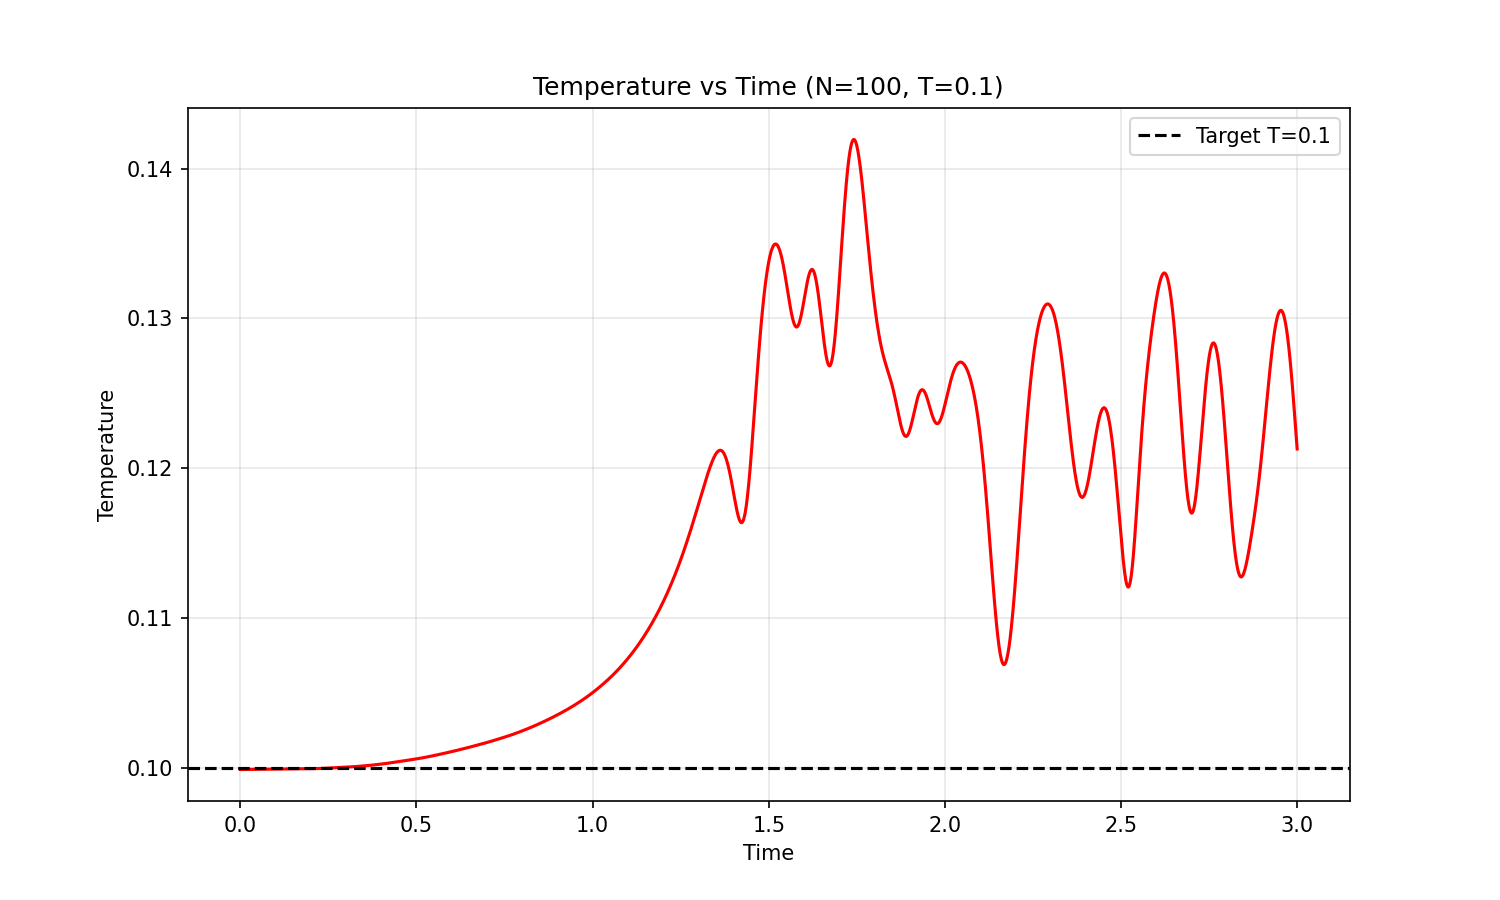
\includegraphics[width=\textwidth]{media/temp_N100_T0.1.png}
		\caption{N=100 particles with T=0.1}
		\label{sfig:nvt_temp_N100_T01}
	\end{subfigure}%
	~
	\begin{subfigure}{0.5\textwidth}
		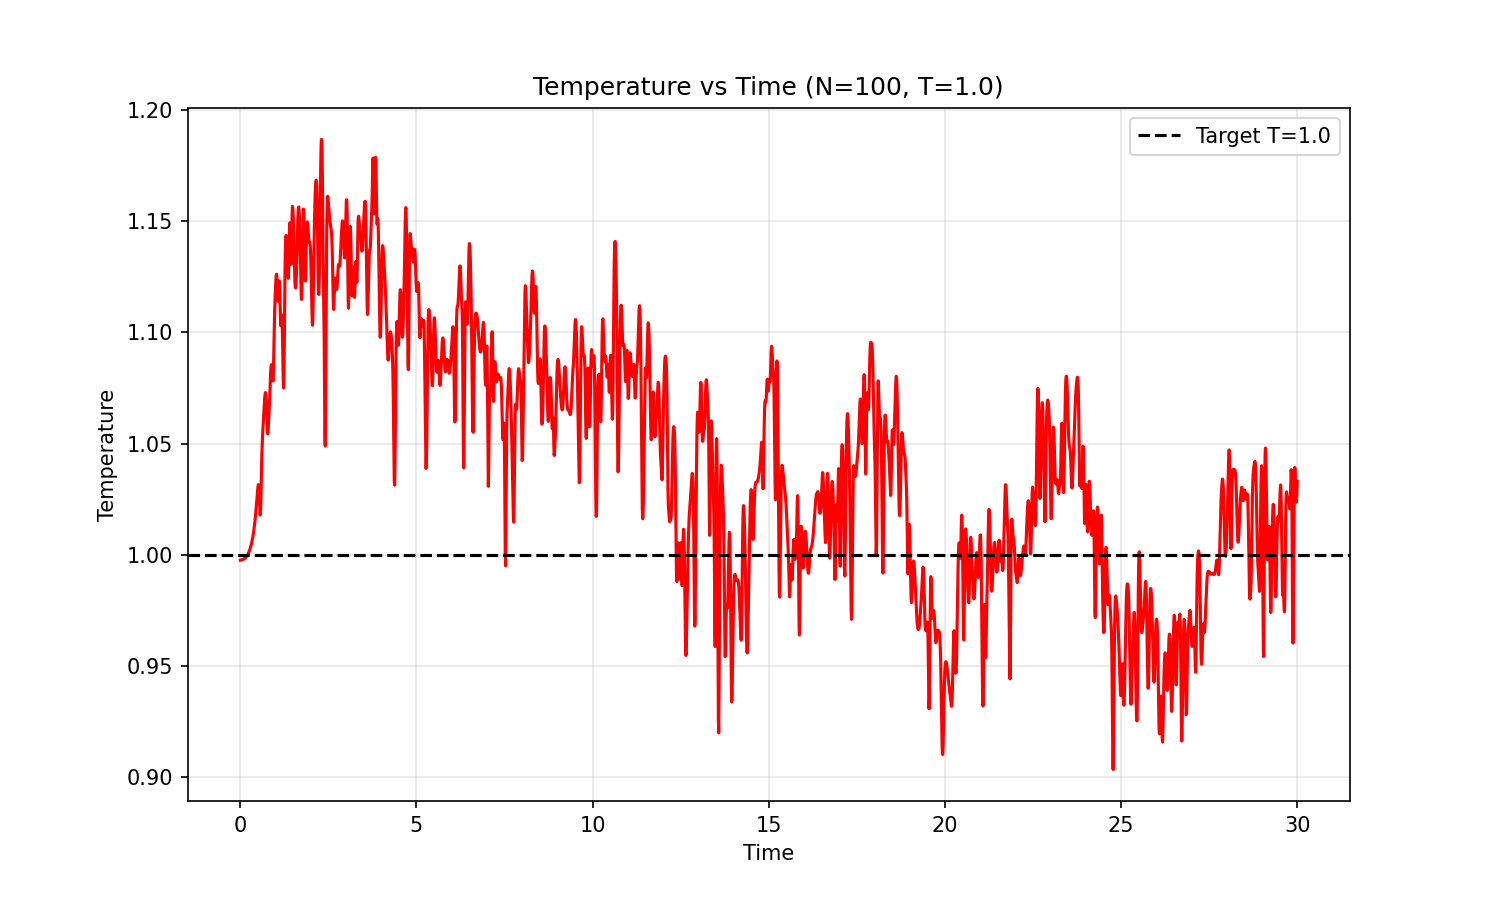
\includegraphics[width=\textwidth]{media/temp_N100_T1.0.png}
		\caption{N=100 particles with T=1.0}
		\label{sfig:nvt_temp_N100_T10}
	\end{subfigure}%
	\\
	\begin{subfigure}{0.5\textwidth}
		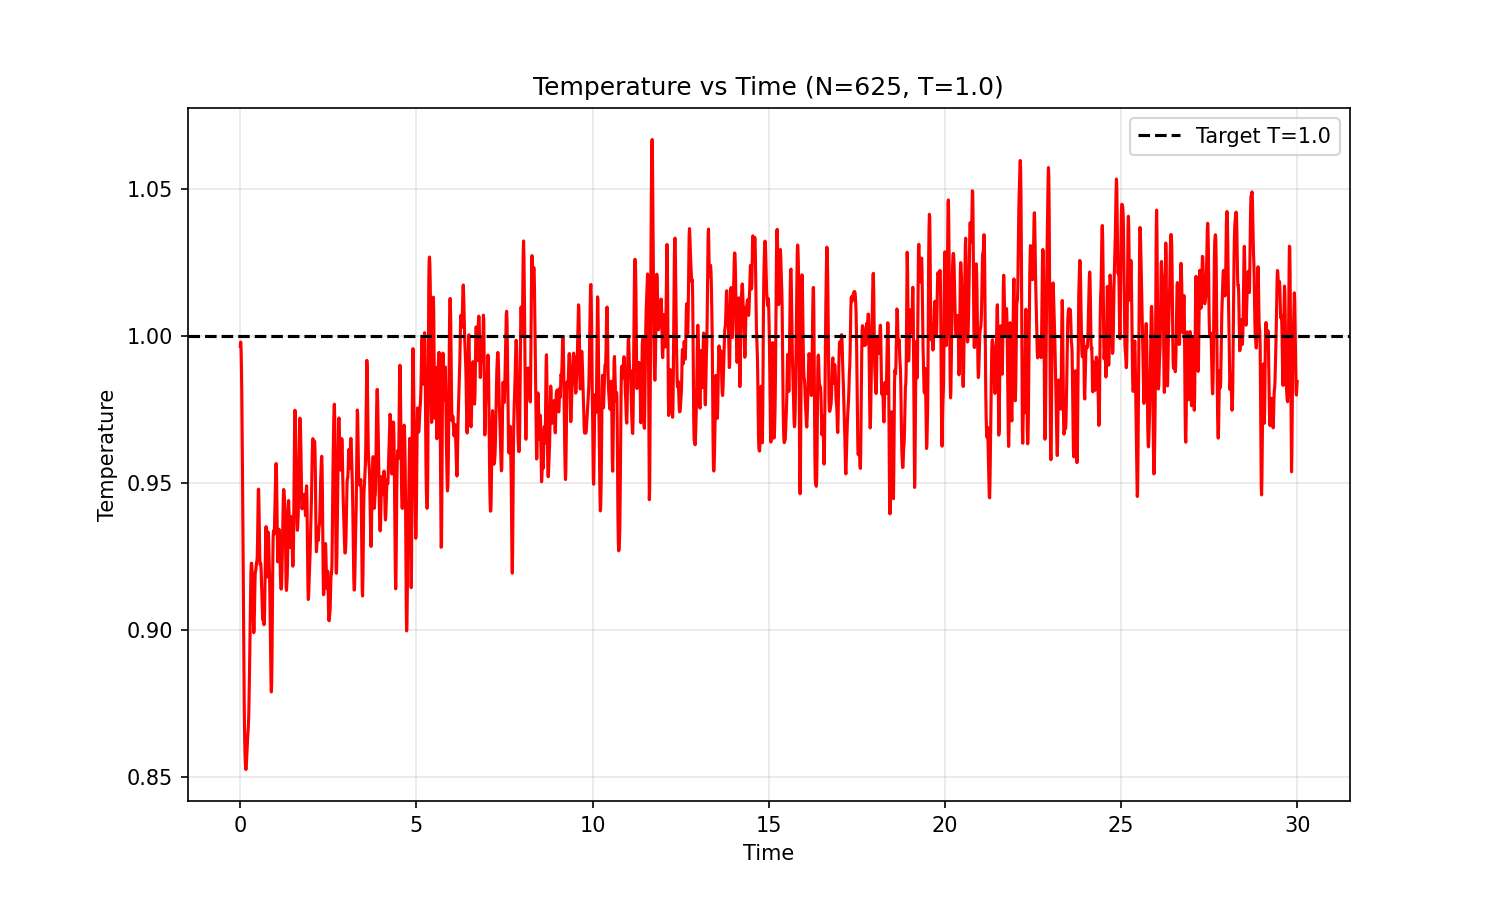
\includegraphics[width=\textwidth]{media/temp_N625_T1.0.png}
		\caption{N=625 particles with T=1.0}
		\label{sfig:nvt_temp_N625_T10}
	\end{subfigure}%
	~
	\begin{subfigure}{0.5\textwidth}
		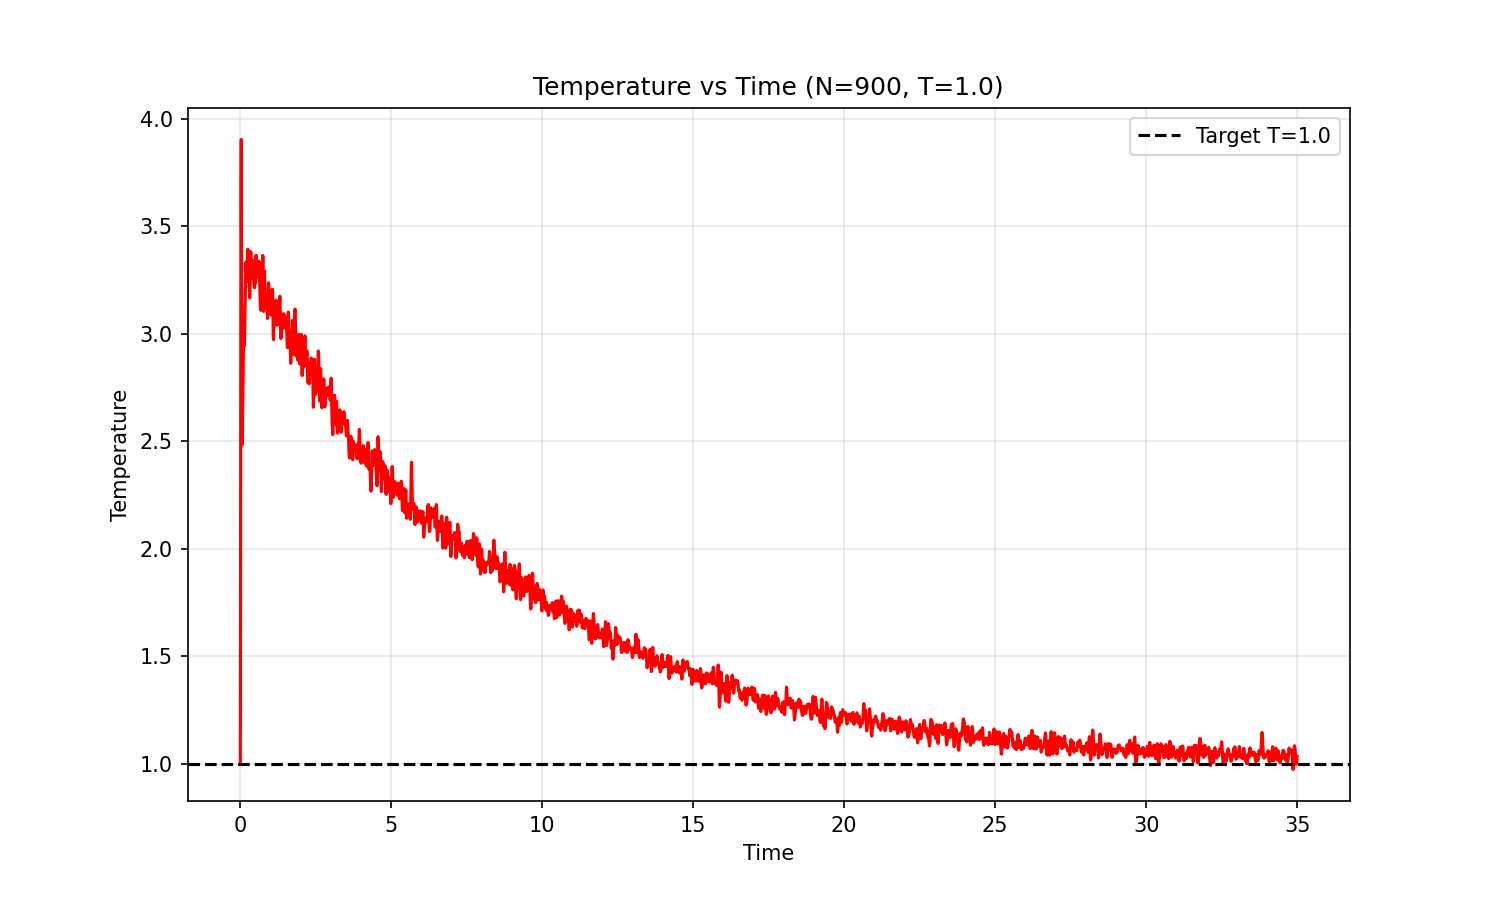
\includegraphics[width=\textwidth]{media/temp_N900_T1.0.png}
		\caption{N=900 particles with T=1.0}
		\label{sfig:nvt_temp_N900_T10}
	\end{subfigure}%
	\caption{\textbf{Temperature Regulation in NVT Ensemble} 
	Temperature evolution for different system configurations using the Berendsen thermostat.}
	\label{fig:nvt_temperature}
\end{figure}
\begin{figure}[H]
	\centering
	\begin{subfigure}{0.5\textwidth}
		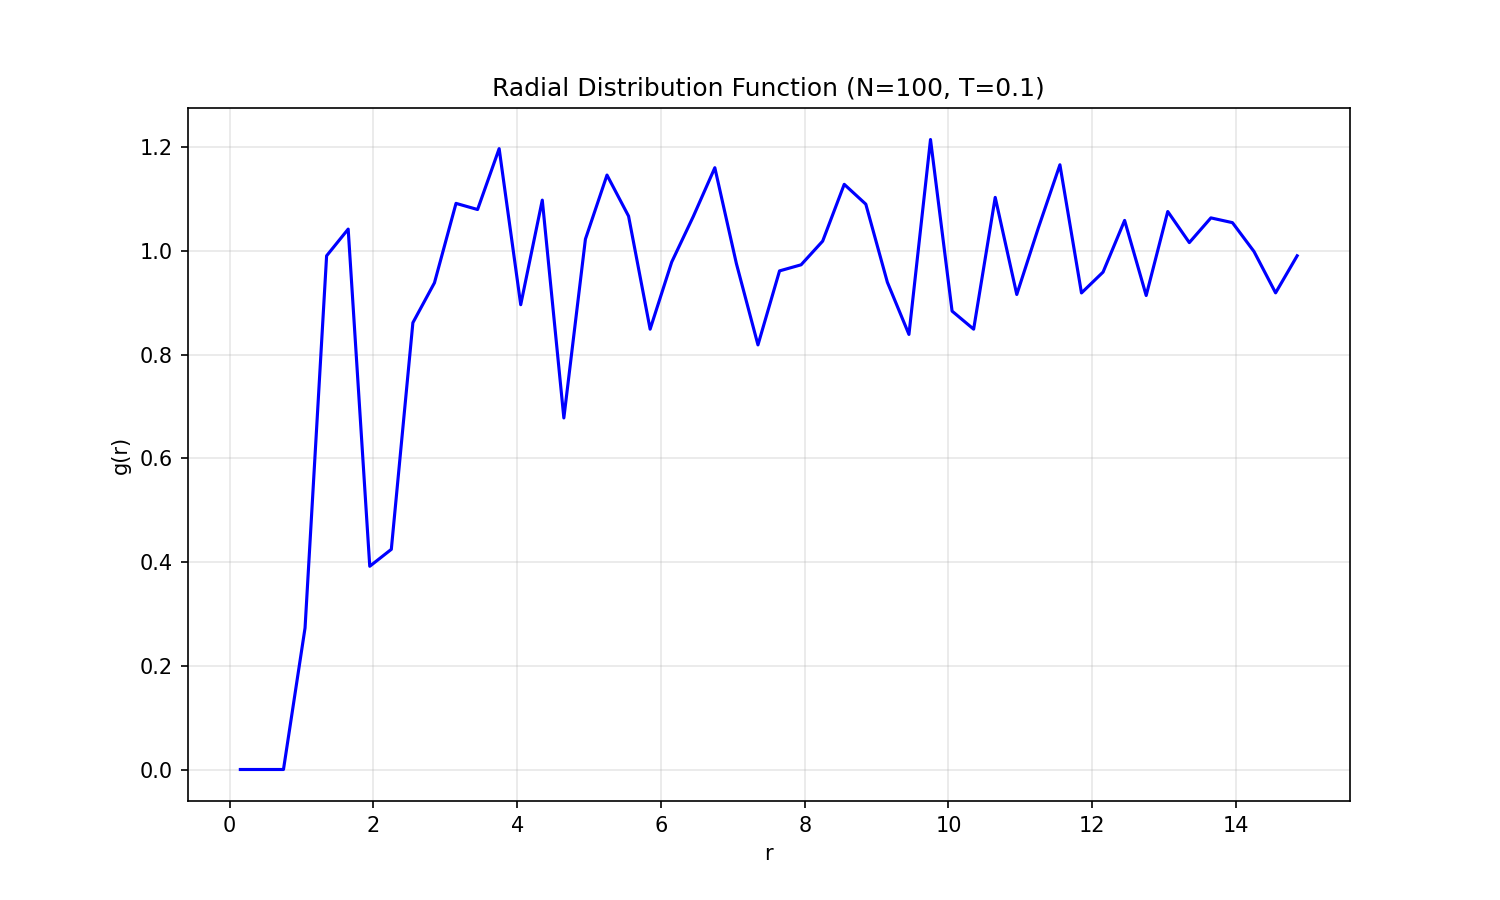
\includegraphics[width=\textwidth]{media/rdf_N100_T0.1.png}
		\caption{N=100 particles with T=0.1}
		\label{sfig:nvt_rdf_N100_T01}
	\end{subfigure}%
	~
	\begin{subfigure}{0.5\textwidth}
		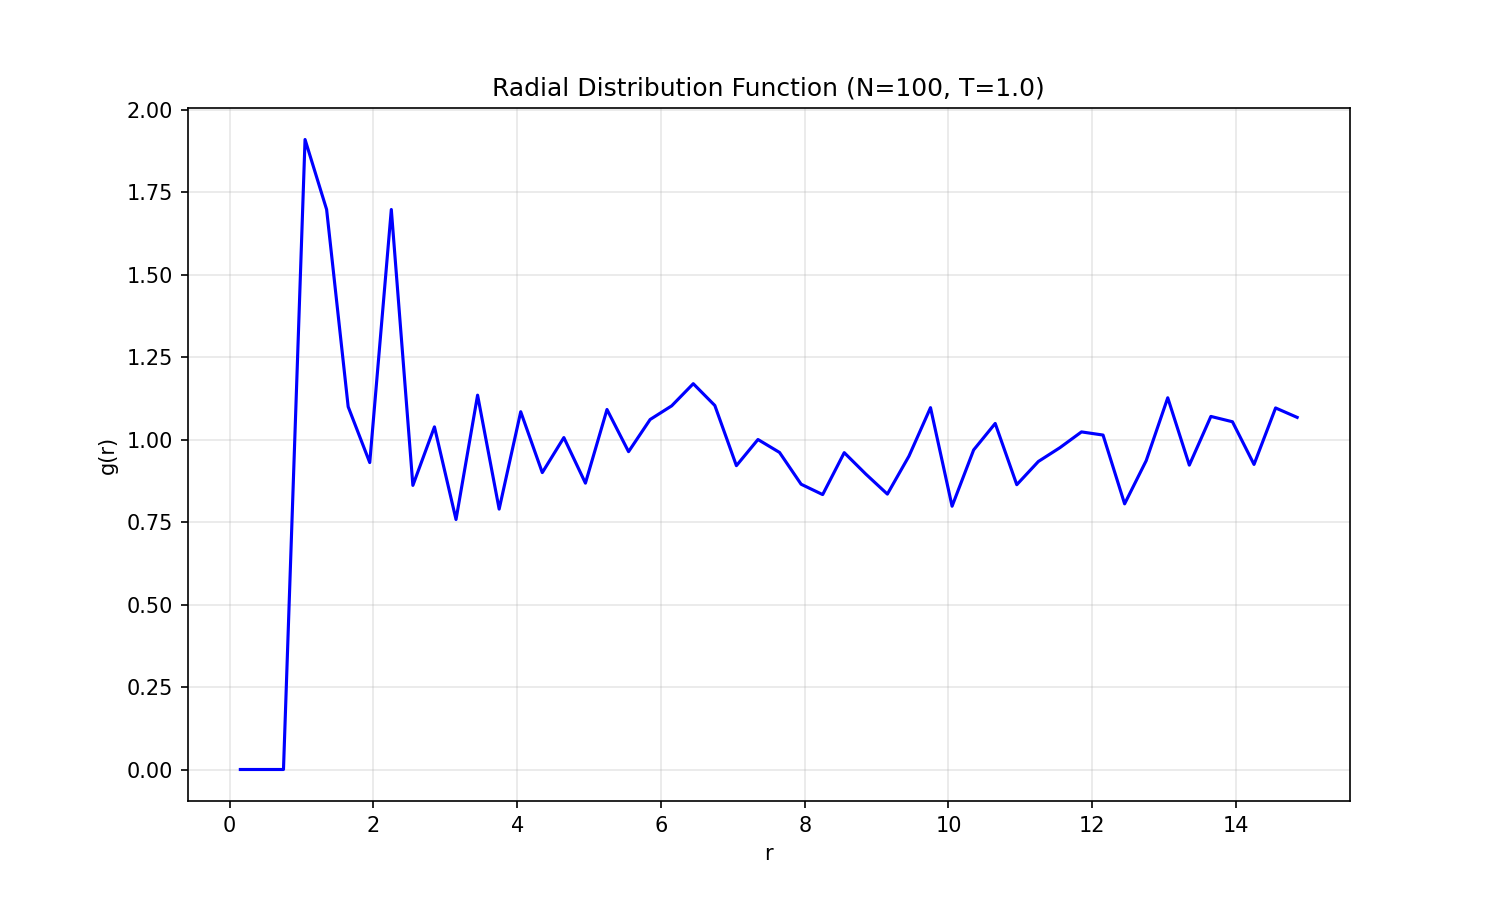
\includegraphics[width=\textwidth]{media/rdf_N100_T1.0.png}
		\caption{N=100 particles with T=1.0}
		\label{sfig:nvt_rdf_N100_T10}
	\end{subfigure}%
	\\
	\begin{subfigure}{0.5\textwidth}
		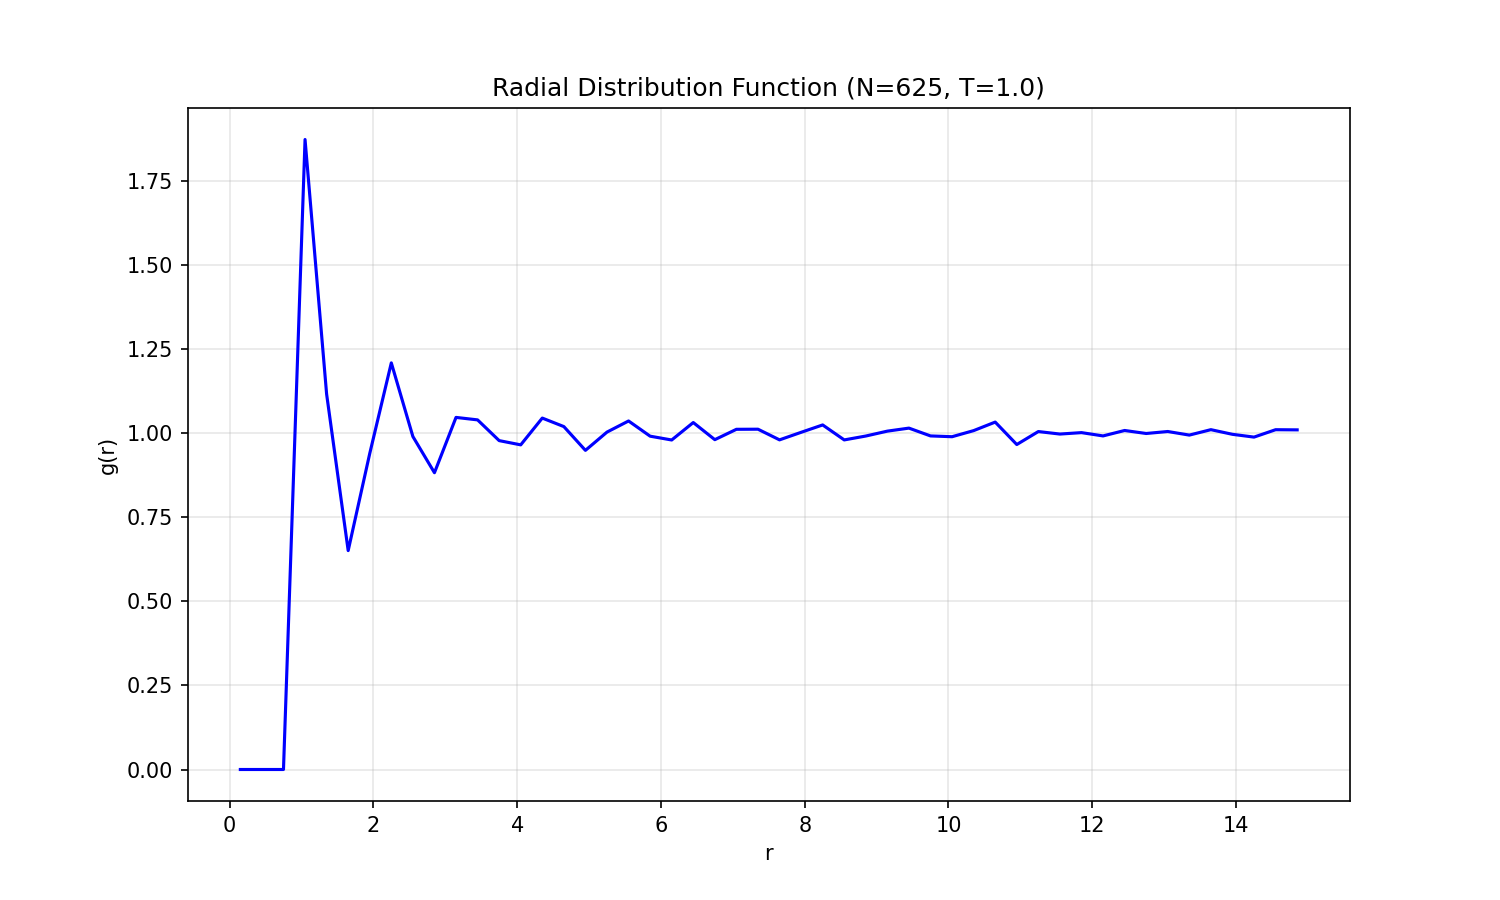
\includegraphics[width=\textwidth]{media/rdf_N625_T1.0.png}
		\caption{N=625 particles with T=1.0}
		\label{sfig:nvt_rdf_N625_T10}
	\end{subfigure}%
	~
	\begin{subfigure}{0.5\textwidth}
		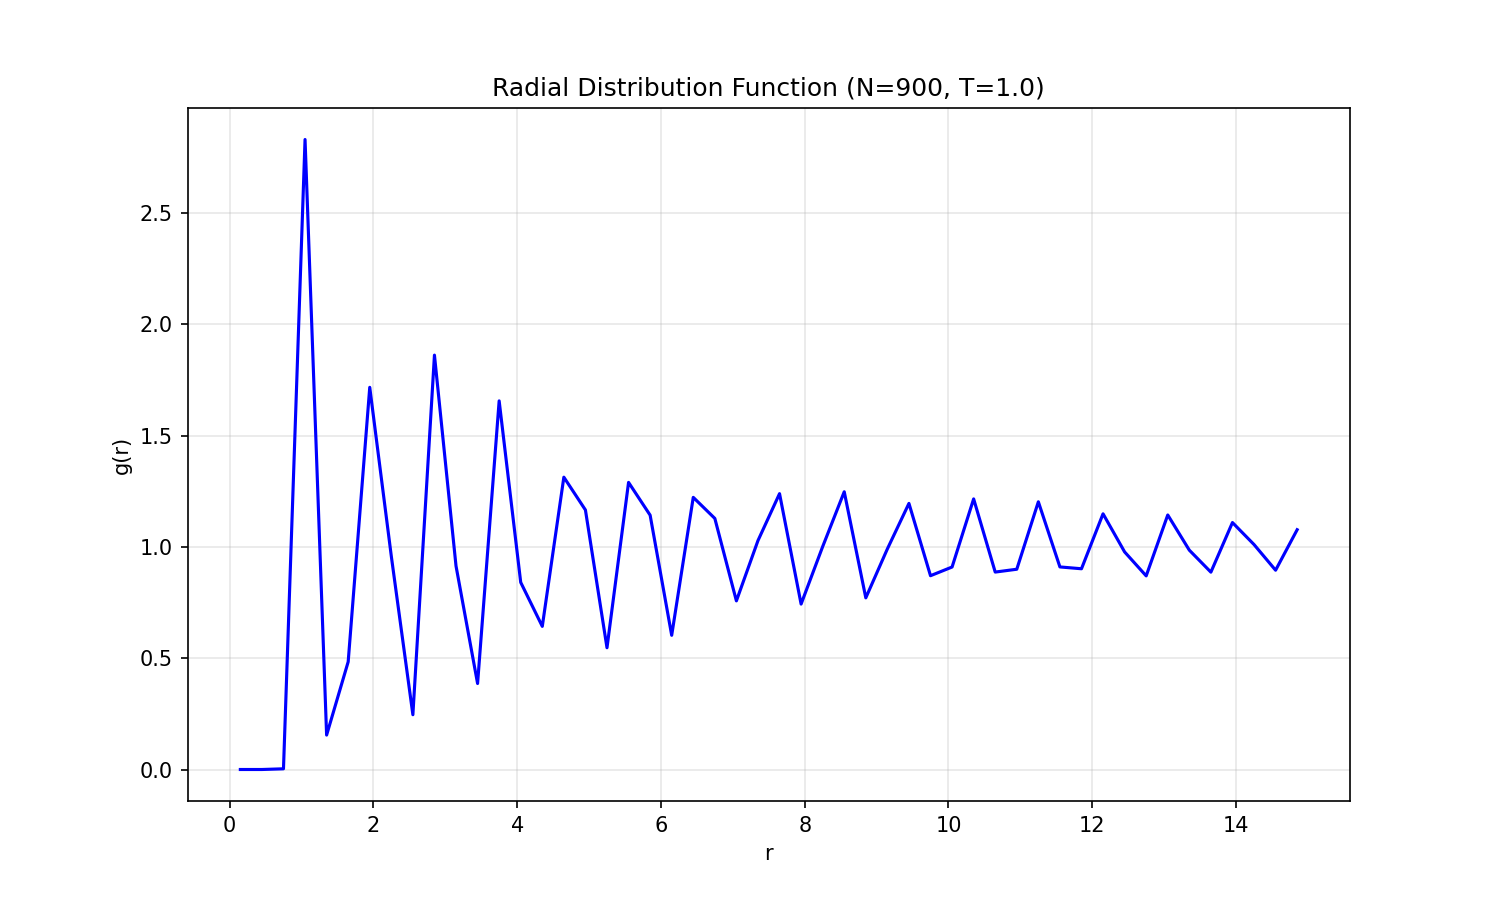
\includegraphics[width=\textwidth]{media/rdf_N900_T1.0.png}
		\caption{N=900 particles with T=1.0}
		\label{sfig:nvt_rdf_N900_T10}
	\end{subfigure}%
	\caption{\textbf{Radial Distribution Functions in NVT Ensemble} 
	Radial distribution functions for different system configurations}
	\label{fig:nvt_rdf}
\end{figure}

\section*{Conclusion}
